\documentclass[12pt, letterpaper]{article}
\usepackage[utf8]{inputenc}
\usepackage[margin=1in]{geometry}
\usepackage{acronym} 
\usepackage{graphicx}
\usepackage{amsmath}
\usepackage{booktabs}
\usepackage{listings}
\usepackage{subfig}

\setlength{\parskip}{1em}
\setlength{\parindent}{0em}
\usepackage{float}
\usepackage{multirow}
\usepackage{amsmath}
\usepackage{amssymb}
%\renewcommand{\labelenumii}{\arabic{enumi}.\arabic{enumii}}
%\renewcommand{\labelenumiii}{\arabic{enumi}.\arabic{enumii}.\arabic{enumiii}}
\renewcommand{\labelenumiv}{\arabic{enumi}.\arabic{enumii}.\arabic{enumiii}.\arabic{enumiv}}
\usepackage[
backend=biber,
style=ieee,
]{biblatex}
%\usepackage[hidelinks]{hyperref}
\usepackage{hyperref}
\usepackage{footnote}
\usepackage{longtable}
\usepackage{graphicx}
\graphicspath{ {images/} }
\usepackage[nottoc]{tocbibind}

\addbibresource{main.bib}

\begin{document}

\begin{titlepage}
    \begin{center}
        
\includegraphics[]{images/hslu_logo.png}
        \vfill
        
        \huge{Industrial Equipment Energy Efficiency Estimation and Performance Deviation Detection Using IoT Enabled Energy Metering}
        
        \vfill
        
        \large{Gabriel Stechschulte, HSLU MSc. Student, Author} \\[10pt]
        \large{Dr. Braulio Barahona Garzon, HSLU, Lecturer} \\[10pt]
        \large{Antoine Finck, CLEMAP, Co-Lecturer}
        
        \vfill
        
        \large{Submission Date: June 3rd, 2022} 
        
        \vfill
        
        A Master Thesis submitted as a requirement of the MSc. Applied Information and Data Science programme from Lucerne University of Applied Sciences and Arts
    \end{center}
\end{titlepage}

\thispagestyle{plain}
\begin{center}
    \large
    \textbf{Abstract}
\end{center}

In a production environment, monitoring the energy consumption of industrial machines is critical in assessing energy efficiency, productivity, and in ensuring the machine in operation does not result in high operating costs. Collaborating with an industrial partner offering metering hardware, data pertaining to the machine's power consumption over a period of $10$ days in a Swiss media and print company is collected and analyzed. Gaussian Processes, a Bayesian non-parametric learning algorithm, is used to model a time series of the energy consumption of the machines. Training a Gaussian Process model on a period of time that represents the ``best operating conditions" and or before any energy intervention process or new component is applied is the ``energy baseline model". Using this model, the next day ahead energy consumption is predicted and compared against the actual values. Using statistical process control methodology, the posterior predictive distribution is used to monitor the degree of severity and uncertainty in instantaneous and cumulative changes in machine energy consumption. An example using the model and process control methodology is given for the paper disposal machine. Furthermore, to prepare the energy baseline model for deployment on the industrial partner's infrastructure, a Docker container is created encapsulating the model's parameters and inference phase. 
\pagebreak

\tableofcontents
\pagebreak
\listoffigures
\listoftables
\pagebreak

\addcontentsline{toc}{section}{List of Data Sources}
\section*{List of Data Sources}
\begin{table}[htbp]
\scalebox{0.90}{
    \renewcommand{\arraystretch}{1.2}
    \centering
    \begin{tabular}{p{8cm}p{6cm}p{2cm}}
    \hline
         Category & Source & Accessed  \\
    \hline
    HIPE Industrial Production Energy & Karlsruhe Institute of Technology & 27.10.2021 \\
    CLEMAP Swiss Media and Printing Production Energy & CLEMAP & 01.12.2022 \\
    \hline
    \end{tabular}}
\end{table}
\pagebreak

\addcontentsline{toc}{section}{List of Abbreviations}
\section*{List of Abbreviations}
\begin{acronym}
       \acro{$A$}{ampere}
        \acro{ACE}{Average Coverage Error}
        \acro{ACF}{autocorrelation function}
        \acro{ADAM}{adaptive moment estimation}
        \acro{API}{application programming interface}
        \acro{BBMM}{Blackbox Matrix-Matrix multiplication}
        \acro{CAS}{compressed air systems}
        \acro{CI}{confidence interval}
        \acro{CLEMAP}{Clever Energy Mapping}
        \acro{CO2}{carbon dioxide}
        \acro{CuSum}{cumulative sum}
        \acro{EDA}{exploratory data analysis}
        \acro{EE}{energy efficiency}
        \acro{EEE}{energy efficiency estimation}
        \acro{EEM}{energy efficiency intervention measure}
        \acro{ETL}{extract transform and load}
        \acro{ETS}{swiss emissions trading scheme}
        \acro{EU}{European Union}
        \acro{EWMA}{exponentially weighted moving average}
        \acro{GAM}{Generalized Additive Model}
        \acro{GHG}{greenhouse gases}
        \acro{GMM}{Gaussian Mixture Model}
        \acro{GPU}{graphical process unit}
        \acro{GPs}{Gaussian Processes}
        \acro{HIPE}{High Resolution Industrial Production Energy}
        \acro{HVAC}{heating ventilation and air-conditioning}
        \acro{$Hz$}{hertz}
        \acro{$I$}{Current}
        \acro{IEA}{International Energy Agency}
        \acro{IP}{internet protocol}
        \acro{IPE}{Institute of Data Processing and Electronics}
        \acro{ISO}{International Organization for Standardization}
        \acro{IoT}{Internet of Things}
        \acro{KIT}{Karlsruhe Institute of Technology}
        \acro{KPIs}{key performance indicators}
        \acro{L}{phase}
        \acro{LCL}{lower control limit}
        \acro{$LocPer$}{\textit{locally periodic}}
        \acro{MA}{moving average}
        \acro{MAPE}{Mean Absolute Percentage Error}
        \acro{MI}{mutual information}
        \acro{MLR}{multiple linear regression}
        \acro{MSE}{Mean Squared Error}
        \acro{MV}{measurement and verification}
        \acro{MW}{Megawatts}
        \acro{NNs}{neural networks}
        \acro{PDD}{performance deviation detection}
        \acro{PI}{prediction interval}
        \acro{$Per$}{\textit{periodic kernel}}
        \acro{QC}{quality control}
        \acro{$RBF$}{\textit{radial basis function}}
        \acro{RMSE}{root mean squared error}
        \acro{RO}{rolling outlier}
        \acro{$RQ$}{\textit{rational quadratic}}
        \acro{SPC}{statistical process control}
        \acro{STL}{seasonal-trend-loess}
        \acro{SVM}{support vector machine}
        \acro{UCL}{upper control limit}
        \acro{$V$}{Voltage}
        \acro{VAR}{reactive power}
        \acro{VAV}{variable air volume}
        \acro{VM}{virtual machine}
        \acro{$W$}{Watts}
        \acro{WEC}{World Energy Council}
        \acro{a.c}{alternating current}
        \acro{kW}{kilowatts}
        \acro{kWh}{Kilowatthour}
        \acro{lr}{learning rates}
        \acro{p.f.}{power factor}
        \acro{r-squared}{coefficient of determination}
        \acro{sq.ft}{square foot}
\end{acronym}
\pagebreak

\section{Introduction}
\subsection{Motivation}

\subsubsection{Industry Partner - CLEMAP}
This thesis is in collaboration with \ac{CLEMAP}\footnote[1]{https://en.clemap.ch/}, a company offering hardware in the form of energy metering sensors for a wide range of electrical appliances and equipment. Complementing their hardware, CLEMAP also offers software products in the form of a data management platform and a software application to provide their customers with the metering data measured by their sensors to act as a basis for analysis, and support and device management.

CLEMAP’s sensors belong to \ac{IoT}, an emerging technology consisting of sensors embedded in physical objects that are linked through wired and wireless networks (routers), often using the \ac{IP}, e.g. using an IP address. In Industry 4.0, these IoT devices are enhancing the metering and sub-metering capabilities of industrial equipment and production processes by collecting not only granular, multi-measurement historical data sets, but also streaming data not previously available for real-time analysis \cite{iot-1}. CLEMAP's meters have the ability to collect a range of information such as \ac{$V$}, \ac{$I$} in \ac{$A$} ($40A$ to $6$kA), \ac{$P$}, \ac{$PF$}, \ac{$Q$}, and \ac{$S$} on each phase of a three phase load at a frequency of $12$ \ac{Hz}. 

With the advancements in sensor technology and increasing availability of large quantities of power-usage and energy consumption data from industrial equipment and commercial production, CLEMAP is looking to expand upon their portfolio of software based services, utilizing IoT, into \ac{EEE} based tools that analyze and monitor energy consumption and identify equipment or processes where energy is ``wasted" and or ``deviating" from their expected behavior.

\subsubsection{Monitoring Energy Efficiency}

First and foremost, what is \ac{EE}? The terminology of EE is broad and definitions can differ from organization to organization and by economic sectors. The \ac{ISO} defines energy efficiency as a ``ratio or other quantitative relationship between an output of performance, service, goods or energy, and an input of energy" \cite{ISO} while the \ac{IEA} and the \ac{WEC} defines energy efficiency as a ``reduction in the energy input of a given service or level of economic activity" \cite{iea-wec}. In the ISO definition, EE is a quantitative measure between an output and input \textit{as is}. Subsequently, the IEA and WEC defines EE as a quantitative measure \textit{given} a reduction in the energy input.

In the organization definitions stated above, EE involves analyzing inputs and outputs which can be difficult in practice as it is not always clear what is defined or measured as an output. As well, smart meters are only logging the energy inputs that the physical device consumes. In this thesis, EE is defined as the amount of energy the equipment or production process consumes \textit{as is} for a given time period with respect to a baseline. It is important to note that in this work, the output of a machine is unknown.  

Energy managers cite a number of benefits attributable to energy metering and monitoring. Fundamentally, they stem from the “you cannot manage what you do not measure” adage \cite{3M}. Building off of this adage, in regard to industry 4.0 and CLEMAP's ambitions, the motivation is to develop an energy consumption baseline for a subset of machines being monitored by CLEMAP's sensors. Being able to accurately model the underlying physical process of a machine is critical to assessing EE and productivity metrics. The development of a model prior to any energy intervention project, new production process or machine components is called an energy baseline model as it establishes an energy consumption baseline / benchmark \textit{as is}. 

With the energy baseline model, at a certain time point, a machine's energy consumption is predicted and then compared to the actual measured value. The difference between the prediction and actual value can be monitored and analyzed over time. Thus, creating value add in assuring the machines that are in production do not cause excessive negative externalities such as high operating costs \cite{eea}, and are operating nominally. Additionally, a well established benchmark can help companies measure and improve their performance not only within the organization, but also to compare with benchmarks established by similar firms in their industry.

\subsubsection{Machine Performance Deviation}

Subsequently, in industry, once you have established a benchmark, and as a production manager or engineer wanting to employ better energy management practices, you want to know if a piece of machinery is deviating away from the benchmark. Complementing the energy baseline model, \ac{PDD} can provide such information with the production manager's domain expertise by detecting if a machine is in an abnormal state, that is, consuming more or less energy than what was expected—compared to the benchmark. Not only can this provide insights into emerging patterns of excessive energy consumption, but it can also provide insights into machine degradation or failure \cite{online-fault-monitoring}. The economic aspect in the context of the equipment life cycle, for just maintenance and support for machine tools, accounts for 60 to 75 percent of the total life cycle cost \cite{econ-costs}. Therefore, PDD can complement the energy baseline model throughout the entire machine life cycle.

\subsubsection{Switzerland Energy Policy}
In the Swiss industrial sector, large energy consuming and \ac{GHG} intensive companies are required to participate in the \ac{ETS}, an accounting system to ensure companies have complied with statutory obligations and to auction off emissions. This system was introduced in 2008 and merged with the \ac{EU} ETS in 2020, along with a \ac{CO2} levy in order to curb GHG \cite{carbon_trading}. Larger companies which are not regulated by the ETS can enter into an agreement with the Federal Office, the canton, or third-party government mandated energy agencies to commit themselves to reduce GHG emissions; ultimately allowing them to be exempted from the CO2 levy and to obtain full or partial refund of the renewable energy network surcharge \cite{optional}. Demand side policy is motivating businesses to employ better energy management practices to not only reduce CO2 emissions, but to also reduce operating costs in the short and long run. 

\subsection{Problem Statement}

Per \hyperlink{subsection.1.2}{Section 1.2}, the development of an energy baseline model forms the foundation for monitoring machine energy efficiency and for identifying when a machine is deviating from nominal behavior. Using data measured with CLEMAP's smart energy meters, how can an energy baseline model be utilized to monitor energy efficiency over time and also detect deviations in machine performance?

\subsection{Research Questions}

In a study leading up to this thesis, a list of plausible research questions were outlined. However, conclusions for every research question were not reached due to time constraints and or focusing on tasks of higher priority. Therefore, below, a list of the relevant research questions to this report are outlined. 

\begin{enumerate}

    \item Smart energy meters only provide information in regard to inputs used by a piece of equipment and without access to ``output" data from the sensors, how can a baseline energy efficiency or benchmark be estimated from energy data alone? Furthermore, how frequently should this benchmark be updated?
    
    \item Could additional data be added or engineered to enhance the solution to research question one such as production data, financial information, temporal aggregations, maintenance logs or weather data?
    
    \item Upon addressing research question one, can performance deviation detection methods, on top of energy efficiency estimation, be implemented to ensure benefits to that particular piece of equipment in the production process life cycle?
    
    \item What information from the results of the algorithms, hypothetically, needs to be transmitted back to the production manager or equipment operator in addressing questions one and three so they can make informed production actions?
    
\end{enumerate}

In Appendix \ref{appendix:c}, a full list of the research questions identified in the preliminary study are outlined. Furthermore, in \hyperlink{section.8}{Section 8}, a reflection on the full list of research questions is given.

\subsection{Project Tasks}

To address the problem statement and research questions stated above, the following main tasks are outlined:

\begin{itemize}
    \item Identify equipment being metered by CLEMAP where an energy baseline model can be applied.
    
    \item With the measurement data, perform a series of experiments to model the equipment from the bullet point above, using a hypothetical reporting period and perform predictions one day ahead.
    
    \item Assess the quality of the model using deterministic and probabilistic evaluation metrics and select the best performing model according to those metrics—this model is then the energy baseline model.
    
    \item Use \ac{SPC} charts to monitor EE over time, and to visualize and detect periods of deviations in performance. 
    
    \item To prepare for a prototype deployment on CLEMAP's infrastructure and environment, create a docker container of the trained energy baseline models.
\end{itemize}

\subsection{Organization of Thesis}

With the introduction, motivation, problem statement, and research questions now set, the remainder of the thesis is organized as follows: \hyperlink{section.2}{Section 2} gives an overview and application of methods pertaining to EEE and PDD in industry. In \hyperlink{section.3}{Section 3}, building off of the related work, the methodology used in this thesis is presented along with the evaluation metrics to assess the quality of the model. Furthermore, advantages and disadvantages of the proposed methodology are given in \hyperlink{subsection.3.4}{Section 3.4}. Then, in \hyperlink{section.4}{Section 4}, two data sets are introduced where an example of an \ac{EDA} workflow is given for a particular machine within the CLEMAP data set. Also, the similarity and differences between the open source and CLEMAP data is given. With the data set and proposed methodology now given, \hyperlink{section.5}{Section 5} contains results and a decomposition of the energy baseline model is described. Subsequently, in \hyperlink{section.6}{Section 6}, monitoring EE and performing PDD using the energy baseline model is explained using a paper disposal machine. In \hyperlink{section.7}{Section 7}, an overview of machine learning deployment and operations is given. In this overview, container technologies are discussed, namely Docker, and a Docker container is developed for the Gaussian Process models. Lastly, \hyperlink{section.8}{Section 8}, provides a summary of the main results, answers to the research questions, and comparison and next steps of the current research is outlined.
\pagebreak

\section{Background and Related Work}
\subsection{Chapter Overview}

\subsection{Overview of Energy Efficiency Estimation Methods}

Regarding the energy domain, various applications can benefit from a more complex data analysis. For instance, most of the different approaches available in literature to monitor and control energy performance in industrial plants share the same main phases [25,26]: measurement plan and data collection, baseline definition, implementation of control over time through comparison between the baseline, and monitored energy consumption


Process control and performance monitoring are other fields interested in the innovation brought by data analytics tools. For instance, some data-driven models are used to give online estimation of key variables that, due to technical or economic limitations, would be too difficult to measure otherwise [60,61], while other models are used to perform process monitoring in order to detect anomalies [62].

The typical method(s) used. i.e., statistical models (regression). Typical applications in industry are usually related to energy consumption at an aggregate level, i.e., building level

The baseline model can be defined as the energy characterization of the starting situation, and its role is fundamental in the assessment of energy savings. 

\subsection{Estimating and Monitoring Energy Efficiency in Industry}

In the literature, there is a vast amount of research and applications on electrical load forecasting. However, given our definition of EE and goal of developing an energy baseline model, the focus in this thesis is on operationalizing the predictions to monitor EE. In industry, this is often the difference between actual energy consumption versus the baseline model predictions. Namely, at predefined time points in the future, $x_{t+n}$, the equipment's input is predicted using the baseline model and is then compared to the actual result when the process is measured at that time step $x_{t+n}$ \cite{tightening}. 

Trager et.al \cite{tightening} used statistical process control (SPC), a technique often used in manufacturing in order to determine whether a process is changing based upon recent measurements. Using six months of data gathered from two commercial buildings in different locations, a seasonal-trend-loess (STL) regression model was developed to predict one hour ahead for each time step. The entire prediction is then moved ahead one hour, so that at each time step in the procedure, one hour of data is predicted. The six months of training data acts as the baseline reporting period in which future predicted energy consumption is analyzed against. Then, using the residuals—the difference between the predictions and actual values—the authors use control charts to monitor EE and analyze deviations in building consumption which is talked about more in \hyperlink{subsection.2.5}{Section 2.5}. 


Benedetti et al. \cite{cas} in a case study with a pharmaceutical manufacturing plant demonstrated the importance of monitoring and controlling energy performance in compressed air systems (CAS) using novel methodology based on meter data and a energy baseline definition using multiple linear regression (MLR) and control charts (see \hyperlink{subsection.2.5}{Section 2.5}). To model the baseline energy performance of the system, a baseline reporting period of one year at $15$ minute intervals taking into account other independent variables such as compressed air production, external temperature, external humidity and pressure is chosen which displays the \textit{best} operating performance of the CAS. Then, using this reporting period, a regression model is developed which acts as the energy baseline model. In order to monitor the energy performance, the authors evaluate the residual between actual energy consumption and the prediction of the baseline model. 

Granderson et al. \cite{lawrence-lab} used two months of electrical load data (August—September) from a small office building complemented with outdoor air temperature to train an energy baseline-modeling agent. Then, the model was used to predict the load for the next two months (October—November). For the first three weeks, the root mean squared error (RMSE) of the hourly load is $1.6$ kilowatts (kW). Then, in the subsequent weeks, the RMSE doubled to $3.2$ kW. Investigation into this new behavior showed that the building had switched into a "heating mode" at the end of October. The building manager had stated this should not happen due to the warmer weather, and as a result, a new HVAC control change was implemented to deter these type of events from happening. 

Nikula et al.\cite{boiler} compared actual boiler efficiency in power stations with its expected efficiency which is an estimate of the highest historical efficiency in the corresponding process state based on multiple linear regression (MLR). The process state is a particular state which is defined as a function of the variables selected using mutual information (MI). Two industrial boilers were analyzed with a capacity of $300$ $\text{MW}_{th}$ and $160$ $\text{MW}_{elec}$, and $220$ $\text{MW}_{th}$, respectively. Each boiler's time series was sampled at an interval of $1$hr. Boiler one included $143$ variables, trained on $810$ hours of data, and was tested (monitored) using $70$ hrs. Boiler two included $125$ variables, trained on $72.5$ hrs, monitored using $3.5$ hours. Using MI, the top two features were chosen and were discretized. The step size in the discretized feature represents a process state. Therefore, in the MLR model, the dependent variable represents the expected efficiency and the features step sizes define the process states. The difference between the actual and expected efficiency was monitored using control controls which is talked about in \hyperlink{subsection.2.5}{Section 2.5} and the two features chosen using MI were analyzed as a potential root cause of deviations.

Benedetto et al \cite{data-driven-MV}, in another application, using metered data from three commercial buildings, complemented with outdoor weather data and binary indicators of holidays, developed an energy baseline model to compare the energy consumption before and after an energy efficiency intervention measure (EEM). Daily load profiles were first identified through the means of a Gaussian Mixture Model (GMM). Then, a Generalized Additive Model (GAM), using the load profiles of the previous seven days, outdoor temperature, sun altitude, wind speed, and a holiday flagging variable is used to model the electricity consumption. This baseline model is then used to compute the counterfactual energy consumption, i.e., the predicted energy consumption if no EEM had taken place. Using the proposed methodologies, upon the EEM in the commercial building, the model achieved an RMSE of $13\%$, $9.1\%$, and $7.8\%$, and predicted a decrease in consumption (kWh) of $8.6\%$, $10.9\%$, $8.3\%$ for building $1$, $2$, and $3$, respectively.

\subsection{Overview of Performance Deviation Detection Methods}

In the previous section, \cite{tightening}\cite{cas}\cite{boiler}, had used a form of charting, built off of the baseline model, to identify when a machine or building was deviating from benchmark efficiency. In industry, this charting is often called SPC, or quality control (QC), and monitors the residuals from the baseline model to measure the statistical significance of the actual energy use deviating from the predicted energy use. Thus, using SPC charts, operators and or production managers of the equipment can gain insight into EE over time and near real-time current deviations in performance.

However, as the field of PDD is vast, it must be acknowledged that analyzing the residuals from regression models is not the only way to perform PDD. Rather, it is a natural extension of time series regression models. Other techniques, primarily using classification and clustering methods, have been proposed and used to perform PDD which will be briefly described here.

Zhang et al. \cite{gas-turbine-faults} used Gaussian mixture model (GMM) techniques to provide recognition of operational states, extraction of load profiles, and to detect emerging faults for industrial turbines. To detect emerging faults, a normal operation state was recognized using a Bayesian GMM technique. Then, with this normal operation cluster a GMM was used to define an ellipse boundary to the cluster and when a new data point fell outside of the ellipse boundary it was identified as a fault. This method, which is now in production, allows the production managers and engineers to analyze, in real time, the performance of their equipment. Gallagher et al. \cite{intelliMAV} implemented a clustering based PDD in the framework of M&V to maintain energy savings. Du et al. \cite{fault-HVAC} combined ANNs to detect abnormalities in the energy consumption of heating, ventilation and air-conditioning systems (HVACs) and used subtractive clustering to classify the abnormalities for diagnostic purposes.

\subsection{Performance Deviation Detection Methods in Industry}

As the main motivation in this thesis is centered around the idea of an energy baseline model, below, PDD based on the use of SPC charts is demonstrated.

Using the residuals from the STL model in \cite{tightening}, three control charts—a moving average (MA), rolling outlier (RO), and a dual measure control chart combining the metrics of the MA and RO charts—are used. The MA chart assumes that the mean of the process should be stationary, and computes the mean of the prediction process residual as a two week rolling average. Using this method, an upper control limit (UCL) and lower control limit (LCL) are calculated to determine when a process is "out of control" and is defined as:

$$\text{UCL / LCL} = \mu +/- \frac{3\sigma}{\sqrt{n * w}}$$

where $\sigma$ is the standard deviation of the process up to the time within window $w$, $n$ is the number of samples averaged at each time point, and $w$ is the total number of samples in the rolling window. Points lying outside of the UCL or LCL indicate the process is deviating from the expected behavior. The RO chart calculates the $99\%$ percentile of residuals in the preceding week, with a point being labeled "hard to predict" if the residual lies in the $99\%$. Combining the RO and MA chart allows one to identify a change in mean of the MA chart and corresponding analysis into which point(s) caused the change indicated by the RO chart. This charting methodology flagged a problem with the HVAC system of the building, and upon inspection, the engineer identified excessive overnight cycling of the HVAC system—resulting in unnecessary energy consumption and equipment usage. 

Building off of the MLR model developed in the case study with the pharmaceutical manufacturing plant \cite{cas}, control charts were developed to identify the EE of the CAS over time. In this study, the authors used instantaneous and the cumulative sum (CuSum) of residuals. Instantaneous and the CuSum of residuals is given by,

$$\text{Instantaneous} = \Delta \text{E}(t) = \text{E}_{act}(t) - \text{E}_{pred}(t)$$
$$\text{CuSum} = \Delta \text{EC}(t) = \sum_{t=0}^t\Delta \text{E}(t)$$

where $\text{E}_{act}(t)$ is the actual energy consumption of the system at time $t$ and $\text{E}_{pred}(t)$ is the predicted energy consumption at time $t$. The difference between these two is the residual, whereas the CuSum is the cumulative sum of residuals from $t=0$ to $t=n-1$. In addition, UCL and LCL were also defined similar to \cite{tightening} to determine the significance of the CAS deviations. However, in this case study, the control limits were defined by $2 \sigma * \Delta \text{E}(t)$. 

Using these two control charts, the authors identified three different operating conditions over a time period of one year. The charts were then reviewed by the operators of the CAS where the first two were related to a maintenance and process intervention; respectively. Lastly, the third operating condition represented an evident malfunctioning of a compressor that remained stuck in stand-by for three consecutive days.


The control charts utilized by \cite{boiler} were developed off of the exponentially weighted moving average (EWMA) statistic which provides an indication of the direction of process performance and the symptoms of possible malfunctions.
\pagebreak

\section{Methodology and Evaluation Metrics}
\subsection{Definition and Characteristics of Time Series}

A time series is a sequential set of data points indexed by time $t$ with some output $y$. It is typically defined as a set of vectors $y(t), t = 0, 1, 2,. . .,n$ where $t$ represents the time elapsed and $y$ is the output. A time series is \textit{univariate} if it consists of single variable over equal periods of time. For example, monthly CO2 measurements is a \textit{univariate} time series. Furthermore, more variables may be added to a time series to make it \textit{multivariate}. A \textit{multivariate} time series consists of multiple time-dependent variables where each variable may also have some dependency on other the variables. Time series can be modelled via discrete or continuous time series models. Continuous time series are recorded at every instance of time, even when the measured variable can only take a discrete set of values (company sales, number of unemployed persons). Discrete time series are when observations are taken only at specific times, usually equally spaced, even if the measured variable is a continuous variable. In this thesis, a continuous time series is discretized by aggregating the time series into equally spaced intervals of 10 and 30 minutes upon which the continuous variables \ac{$W$}, $V$, and $I$ are analyzed. 

Within a time series, there are typically four components to be considered which may influence the analysis or modeling. Not all time series contain all four components, and certain models are aimed at modeling time series with only a subset of these components. Thus, the EDA and subsequent model selection are important phases of time series analysis. Below, the main components of a time series are defined.

\textbf{Trend}: A trend is a general tendency of a time series to increase, decrease or stagnate over time \cite{tsa}. For example, global warming, a time series referring to the global temperature, exhibits an increasing trend. 

\textbf{Seasonal}: Seasonality is when a time series is influenced by seasonal factors (e.g., the quarter of the year, the month, or day of the week). Time series longer in duration may have multiple seasonality components. For example, airline data on the number of passengers flying exhibits multiple seasonality—vacation and holiday periods \cite{tsa}.

\textbf{Cyclical}: The cyclical variation in a time series describes data that exhibits rises and falls that are \textit{not of fixed period}. The duration of a cycle depends on the type of industry or business being analyzed. For example, electrical load profiles of residential buildings often exhibit a cyclical pattern as the demand for energy \textit{cycles} throughout the day, but is typically not of a fixed period, i.e., people continue living in the building for a long period of time. 

\textbf{Irregular}: This component is unpredictable. Every time series has some unpredictable component that makes it a random variable. In prediction, the objective is to “model” all the components to the point that the only component that remains unexplained is the random component. This component is also sometimes called the \textit{residual} \cite{tsa}. 

In this thesis, it is expected that the industrial equipment will show a strong cyclical pattern as the loads of the equipment will be influenced by production process schedules; in turn influenced by the ``business week". In \hyperlink{subsubsection.4.1.1}{Section 4.1.1}, an exploratory analysis will be conducted to visualize the components of the machine's time series. 


\subsection{Introduction to Gaussian Processes for Time Series}

\ac{GPs} belong to the family of \textit{Bayesian non-parametric models} and offer a principled, interpretable, and intuitively specified way for conducting probabilistic inference of non-linear time series. Non-parametric methods do not assume a fixed parametric form for the prediction function, but instead try to estimate the function itself (rather than the parameters) directly from the data. 

GPs can be viewed as a generalization of a Gaussian distribution in $\mathbb{R}^n$ to a space of functions. More specifically, a GP is a way to define distributions over functions with the assumption that the function values at a set of $M > 0$ inputs, $f = [f(x_1), . . .,f(x_M)]$, is jointly Gaussian with a mean $(\mu = m(x_1), . . .,m(x_M))$ and covariance $\sum_{i, j} = K(x_i, x_j)$, where $m$ is the mean function and $K$ is a positive definite kernel \cite{pml1Book}. A positive definite kernel is a generalization of a positive definite matrix where the matrix is symmetric and all its eigenvalues are positive. 

Thus, the two central components of a GP are the mean $m(x)$ and covariance kernel function $k(x_i, x_j)$. The former represents the value we expect for our function before seeing the data, and the latter, the beating heart of a GP, specifies the correlation between any pair of outputs and therefore determines the properties of the function that it generates. The kernel allows one to encode prior knowledge about the similarity of the two input vectors $x_i$ and $x_j$, i.e., if we know that $x_i$ is similar to $x_j$, then the model can be encouraged to make the predicted output at both locations $f(x_i)$ and $f(x_j)$ to be similar. As the problem in this thesis is concerned with time series, the informativeness of past observations in explaining current data is a function of how long ago the past observations were observed \cite{roberts_gaussian_2013}. The covariance matrix for a set of locations $x = \{x_1, x_2, . . .,x_n\}$ is defined as:

\begin{equation}
K(x, x') = \begin{pmatrix}
k(x_1, x_1) & k(x_1, x_2) & \dots & k(x_1, x_n) \\
k(x_2, x_1) & k(x_2, x_2) & \dots & k(x_2, x_n) \\
\vdots & \vdots & \vdots & \vdots \\
k(x_n, x_1) & k(x_n, x_2) & \dots & k(x_n, x_n)
\end{pmatrix}
\end{equation}

This means that the entire function evaluation, associated with points in $x$, is drawn from a multivariate Gaussian distribution \cite{roberts_gaussian_2013}:

\begin{equation}
p(y(x)) \sim \mathcal{N}(m(x), K(x, x'))
\end{equation}

where $y = \{y_1, y_2,. . .,y_n\}$ are the dependent function values, evaluated at locations $x_1,. . .,x_n$, $m$ is a \textit{mean function} and $K$ is a kernel function, again evaluated at the locations of the $x$ variables. If one believes there is noise (which there often is) associated with the observed function values $y_i$, then a noise term can be directly incorporated into the covariance function:

\begin{equation}
K(x, x') + \sigma^2I
\end{equation}

where $I$ is the identity matrix since noise is expected to be uncorrelated from sample to sample; hence noise only needs to be added to the diagonal of $K$ \cite{roberts_gaussian_2013}. The $\sigma^2$ is a hyper-parameter representing the noise variance.

A GP with a given \textit{mean function} $m$ and \textit{covariance function} $K$ is a prior that can generate functions; hence the common definition of a GP as a ``prior distribution over functions". Now that the central components of a GP have been laid out, the following describes how to perform inference. To perform inference with GPs from some input (test data) $X_*$ given some training data $D = \{(x_i, y_i)\}$ assuming i.i.d additive Gaussian noise with variance $\sigma_{n}^2$, the prediction and observations are expressed as a joint distribution following the GP prior \cite{roberts_gaussian_2013}:

\begin{equation}
\begin{bmatrix} 
y \\ 
y_*
\end{bmatrix} 
\sim{~} \mathcal{N} (m, \begin{bmatrix} 
K(X, X) + \sigma_{n}^2I & K(X, X_*) \\
K(X_*, X) & K(X_*, X_*)
\end{bmatrix})
\end{equation}

where $y_*$ is some output test data and $X_*$ is the input test points. One can think of the evaluation of test points $X_*$ at new locations as \textit{augmenting} the observed data $X$ with the test data $X_*$ and $y_*$ in the joint distribution. 

With the product rule, one can relate the joint distribution to the conditional distribution to obtain the posterior predictive distribution \cite{pml1Book}:

\begin{equation}
p(f_* | X_*, X, y) = \mathcal{N}(f_* | m_*, \sum_*)
\end{equation}

with mean and covariance given by:

\begin{equation}
m^* = m(x_*) + K(X_*, x)(K(X, X) + \sigma_{n}^2)^{-1}(y - m(x))
\end{equation}
\begin{equation}
\sum_{*} = K(X_*, X_*) - K(X_*, x)[K(X, X) + \sigma_{n}^2]^{-1}K(X, X_*)
\end{equation}

Gaussian Process models have a number of parameters $\theta$ (sometimes called hyperparameters) resulting from the mean and kernel function that must be \textit{marginalized} in order to perform inference. These parameters are talked about in \hyperlink{section.3.3}{Section 3.3}. As a GP is within the Bayesian framework, priors are first assigned to these hyperparameters using distributions utilizing our domain knowledge. Kernel parameters and incorporating expert opinion through the use of the \ac{ACF} is described in \hyperlink{subsubsection.3.3.2}{Section 3.3.2}. Ideally, with prior distributions assigned to the hyperparameters, we would like to use Bayes rule to compute the posterior to find the \textit{most likely} parameters:

\begin{equation}
p(\theta | y) = \frac{p(y | \theta)p(y)}{p(y)}
\end{equation}

However, the marginal likelihood $p(y | \theta)$ is almost always intractable and we must therefore use approximation techniques \cite{pml1Book}. To find the \textit{most likely} hyperparameters, the marginal log-likelihood is maximized through gradient-based optimization and is given by the form:

\begin{equation}
log P(y | X, \theta) = -\frac{1}{2}y^T(K_{y} + \sigma_{n}^2)^{-1} - \frac{1}{2}log|K_{y} + \sigma_{n}^2| - \frac{n}{2} log(2\pi)
\end{equation}

In \hyperlink{subsection.5.1}{Section 5.1}, the experimentation setup pertaining to the type of optimizer used, number of training iterations, and learning rate is given. Although the above is technical, GPs have an intuitive procedure for training and performing inference. First, prior beliefs are encoded using kernel functions.  Second, condition on what data has been observed. Third, optimize the parameters. Lastly, use the posterior predictive distribution for performing inference.

\subsection{Covariance and Mean Functions}

As outlined above, the kernel design is a vital step in GP model design and offers an opportunity to incorporate domain knowledge into the model. Below, a few kernels and their hyperparameters that will be useful in modeling non-linear time series will be introduced and subsequently, an explanation on how to compose kernels through addition or multiplication will be provided.

\subsubsection{Squared Exponential Kernel}

First, the \textit{squared exponential} or \ac{$RBF$} kernel is one of the most widely used kernels for real-valued inputs. Notably, the $RBF$ is a stationary kernel that encodes a high degree of smoothness in the function space \cite{pml1Book}, and hence can be used to design a GP which produces functions that can be smooth,

\begin{equation}
    K_{RBF} = \sigma^2 exp(-\frac{||x - x'||}{2 \ell^2})
\end{equation}

where $\ell$ is the lengthscale and controls the ``wiggliness" of the function and $\sigma^2$ is the overall variance / outputscale  ($\sigma$ is also known as the amplitude) of the function. In Figure \ref{fig:fig1} below, three functions are sampled and visualized from an $RBF$ kernel; each with different length and outputscale values.

\begin{figure}[htp]
\centering
\graphicspath{ {./images/} }
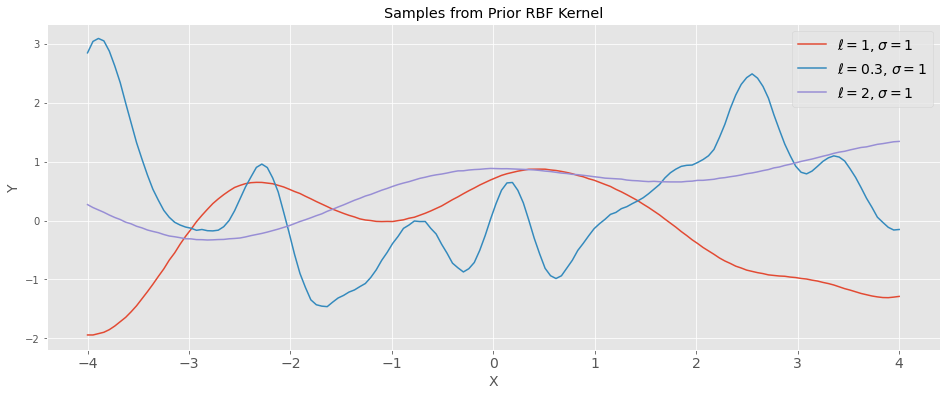
\includegraphics[scale=0.49]{images/samples_rbf_prior.png}
\caption{Three samples, each from an $RBF$ kernel with different hyperparameters denoted by the table legend. Notice how $\ell$ affects the smoothness of the function.}
\label{fig:fig1}
\end{figure}

\subsubsection{Periodic Kernel}

The \ac{$Per$} captures repeating structures \cite{pml1Book}, which can model seasonalities influenced by business cycles and or human behavior. For example, home electricity consumption often displays daily seasonalities. The $Per$ kernel has the form

\begin{equation}
K_{per} = exp(-\frac{2}{\ell^2} sin^2 (\pi \frac{r}{p}))
\end{equation}

where $p$ is the period. Again, $\ell$ and $\sigma^2$ are the lengthscale and outputscale respectively. Figure \ref{fig:fig2} below visualizes the repeating structures of the $Per$ kernel. Important in this thesis is how the period is chosen. In a time series, the correlation between any pair of outputs can be analyzed empirically using the ACF. The ACF compares the time series with itself at a certain lag. Namely:

\begin{figure}[htp]
\centering
\graphicspath{ {./images/} }
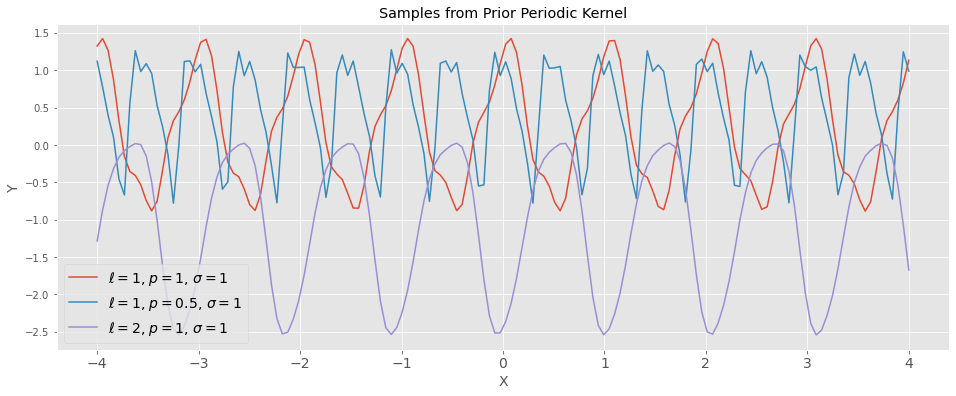
\includegraphics[scale=0.49]{images/samples_periodic_prior.png}
\caption{Three samples, each from a $Per$ kernel with different hyperparameters denoted by the table legend. Notice how $p$ affects the periodicity of the function and $\ell$ affects the ``wiggliness" of the variations.}
\label{fig:fig2}
\end{figure}

\begin{equation}
    \hat{p}(k) = \frac{\sum_{s=1}^{n-k}(x_{s+k} - \bar{x})(x_s - \bar{x})}{\sum_{t=1}^{n-k}(x_t - \bar{x})^2} 
\end{equation}

Thus, using the ACF coefficients, the interval of periods that show significant autocorrelations are chosen as the prior belief for the time series cyclical period length. Increasing the period $p$ increases the distance between repetitions. Figure \ref{fig:fig3} below shows an example of the ACF correlogram for the paper disposal machine and how one can use the coefficients at certain lags as a prior belief for modeling the cyclical component. 

\begin{figure}[htp]
\centering
\graphicspath{ {./images/} }
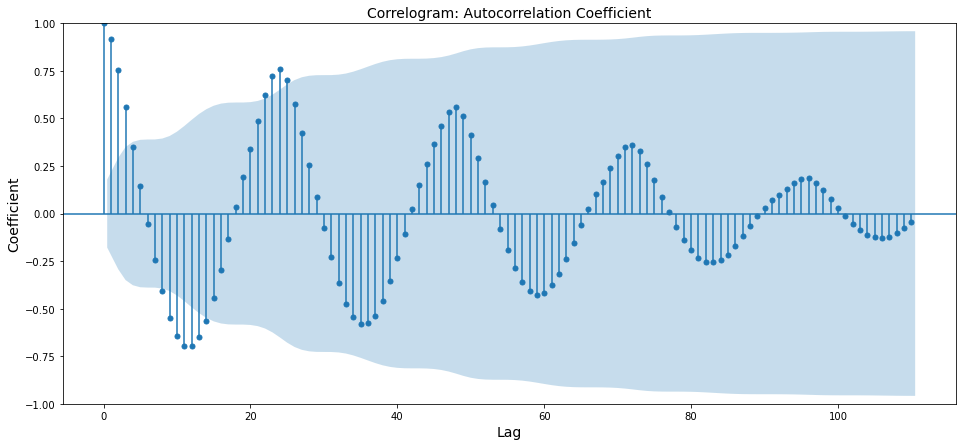
\includegraphics[scale=0.48]{images/entsorgung_acf.png}
\caption{Entsorgung ACF. The time series is discretized and averaged at $1$ hour intervals. Therefore, the ACF shows significant autocorrelations between $10$ and $12$ hours and $22$ and $24$ hours with the remaining lags decreasing in amplitude and significance.}
\label{fig:fig3}
\end{figure}

\subsubsection{Rational Quadratic Kernel}

The \ac{$RQ$} can be interpreted as the sum of many $RBF$ kernels of different lengthscales. Similar to the $RBF$, the $RQ$ kernel encodes smoothness in the function space, but with the additional flexibility of having both local variations and long term variations \cite{gp_prices}. 
\begin{equation}
    K_{RQ} = \sigma^2 exp(1 + \frac{(x - x')^2}{2\alpha \ell^2})
\end{equation}

where $\alpha$, also known as the scale mixture, determines how much local variations from the smaller lengthscales contribute to the overall variation. By using this kernel, one can model non-periodic trends of the underlying physical process and interpret the hyperparameters $\ell$ as either a non-periodic hourly or daily trend depending on how large or small the value of $\ell$ is respectively. Three samples of the $RQ$ kernel are visualized in Figure \ref{fig:fig4}.

\begin{figure}[htp]
\centering
\graphicspath{ {./images/} }
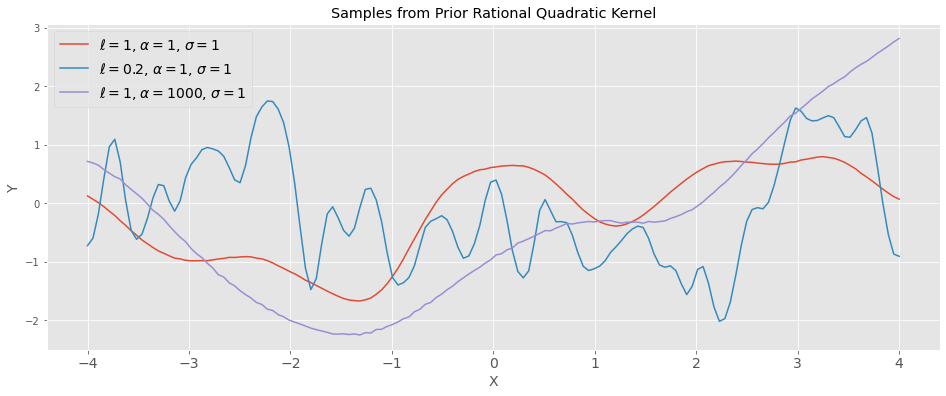
\includegraphics[scale=0.49]{images/samples_rq_prior.png}
\caption{Three samples, each from a $RQ$ kernel with different hyperparameters denoted by the table legend. Notice how $\alpha$ affects the local variations of the function while $\ell$ affects the ``wiggliness" of the variations.}
\label{fig:fig4}
\end{figure}

\subsubsection{Kernel Composition}

Kernels can also be combined through addition and multiplication given the result is a positive definite kernel \cite{pml1Book}. Therefore, by combining kernels, more complex covariance structures can be designed. The addition of two kernels $K_1(x, x')$ and $K_2(x, x')$ is analogous to the probabilistic ``OR" operation, i.e., two points $x_1$ and $x_2$ are considered highly correlated if they are highly correlated in $K_1 \lor K_2$. The multiplication of the two kernels is analogous to the probabilistic ``AND" operation, i.e., two points $x_1$ and $x_2$ are considered highly correlated if they are highly correlated in $K_1 \land K_2$. The resulting kernel given by the addition or multiplication of the two kernels is given by:

\begin{equation}
    K(x, x') = K_1(x, x') + K_2(x, x')
\end{equation}
\begin{equation}
    K(x, x') = K_1(x, x') * K_2(x, x')
\end{equation}

\subsubsection{Locally Periodic Kernel}

In time series analysis, the periodic structure of the underlying function may change and or may not be consistent over time. For example, Figure \ref{fig:fig10} shows a daily repeating cycle that changes its structure over the course of the week. Thus, one may want to incorporate this locally changing periodic structure ``belief" into the kernel design \cite{gp_prices}. To do this, a \ac{$LocPer$} is introduced. The $LocPer$ kernel is a product of the $K_{RBF}$ and $K_{Per}$:

\begin{equation}
    K_{LocPer} = \sigma^2 exp (-\frac{2sin^2(\pi(x - x') / p}{\ell_{Per}^2}exp(-\frac{(x - x')^2}{\ell_{RBF}^2}))
\end{equation}

The periodic component correlates points that are far away from each other, but still in the same phase of a cycle. The $K_{RBF}$ decorrelates the two points and how quickly the points are decorrelated is determined by the hyperparameter $\ell_{RBF}$. Remember, $\ell_{RBF}$ determines the ``wiggliness" of the function; therefore smaller $\ell_{RBF}$ corresponds to faster changing periodic cycles and vice versa. The $K_{LocPer}$ is of use in modeling industrial machine equipment energy consumption as production processes are typically influenced by human behavior. Below, in Figure \ref{fig:fig5}, three samples are generated from a $LocPer$ kernel.

\begin{figure}[htp]
\centering
\graphicspath{ {./images/} }
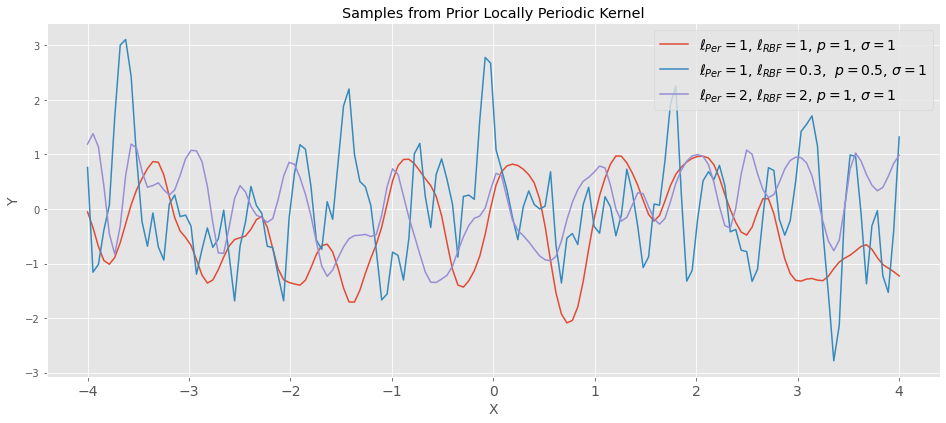
\includegraphics[scale=0.49]{images/samples_locper_prior.png}
\caption{Three samples, each from a $LocPer$ kernel with different hyperparameters denoted by the table legend. Notice how the product of the two kernels results in a periodic structure with variations in each cycle.}
\label{fig:fig5}
\end{figure}

\subsection{Advantages and Disadvantages of Gaussian Processes}

In this thesis, Gaussian Processes for time series was chosen for the advantages to (1) perform non-parametric probabilistic inference to model non-linear time series, (2) allow for an intuitive model interpretation by way of \textit{decomposition} of the kernels, and (3) incorporate background information in the form of \textit{kernel design}.

However, GPs also have disadvantages. The main one being a result of the kernel $K$, that when performing inference and likelihood evaluation, to compute the weights, the method has a computational complexity of $\mathcal{O}(N^3)$. That is, the time complexity is cubic in the number of points $|N|$ \cite{pml1Book}. However, the open source software used in this thesis \cite{gardner2018gpytorch} for implementing Exact Gaussian Processes (ExactGP) is based on \ac{BBMM} \cite{NEURIPS2018_27e8e171} to reduce the time complexity down to $\mathcal{O}(N^2)$. Another disadvantage of GPs is the choice of kernel design. Knowing which kernel to use to model the underlying process and how to compose them can be a challenging task. However, using other people's domain knowledge and other methods such as the ACF makes the task more manageable. 

\subsection{Evaluation Metrics}

To evaluate the performance of the model, the data set is first split into training and testing sets. The training set consists of four days of data where as the testing set consists of one days ($24$ hours) worth of data. Then, as GPs are probabilistic models, to evaluate model quality, not only should the accuracy of the model's predictions be computed, but also how precise the predictions are using the posterior predictive distribution. Thus, deterministic and probabilistic error metrics are used in this thesis. The following metrics are used to evaluate the performance and quality of the model:  \ac{MSE}, RMSE, \ac{MAPE}, \ac{ACE}, and Pinball Loss.

\begin{itemize}
    \item \textit{MSE}: Also known as the average squared loss, measures the average squared distance the predictions are from the actual values. A larger MSE indicates that the data points are dispersed more widely around the mean, whereas a smaller MSE suggests the inverse. In regression, the smaller the MSE, the better. MSE is given by:
    
    \begin{equation}
        \frac{1}{n}\sum_{i=1}^n(\hat{y_t} - y_t)^2
    \end{equation}
    
    where $\hat{y_t}$ is the forecasted value at time $t$ and $y_t$ is the actual value at time $t$. 
    
    \item \textit{RMSE}: Is the square root of MSE. The square root function turns the metric back into the same units as the dependent variable $y$. Again, the smaller the RMSE, the better and is defined as:
    
    \begin{equation}
        \sqrt{\frac{1}{n}\sum_{i=1}^n(\hat{y} - y)^2}
    \end{equation}
    
    where $\hat{y_t}$ is the forecasted value at time $t$ and $y_t$ is the actual value at time $t$. 
    
    \item \textit{MAPE}: Measures the accuracy of the forecast as a percentage and offers an intuitive way to communicate the quality of a model to non-technical audiences. For example,  a $15\%$ MAPE would mean that, on average, the model is off the true value by $15\%$. The smaller the MAPE, the better, and is defined as:
    
    \begin{equation}
        \frac{1}{n}\sum_{i=1}^n \frac{|y_t - \hat{y_t}|}{A_t}
    \end{equation}
    
    where $y_t$ is the actual value at time $t$ and $\hat{y_t}$ is the forecasted value at time $t$. The absolute difference is then divided by the actual value $y_t$ to obtain a scale-independent measure. 
    
    \item \textit{ACE}: Sampling functions from the posterior predictive distribution, one can obtain \ac{PI}. In this thesis, two standard deviations (95\%) is used. ACE measures the proportion of actual values within the PI and is bounded between $[0, 1]$:
    
    
    \begin{equation}
        I_t = 
    \begin{cases}
      1 & \text{if} \quad P_t \in [\hat{L_t}, \hat{U_t}] \\
      0 & \text{if} \quad P_t \notin [\hat{L_t}, \hat{U_t}]
    \end{cases}
    \end{equation}
    \begin{equation}
        UC = \frac{1}{|T|}\sum_{t\inT}I_t
    \end{equation}
    
    where $P_t$ is the actual value at time $t$, and $I_t$ is a binary indicator of whether the PI $ [\hat{L_t}, \hat{U_t}]$ contains $P_t$. Since ACE measures a proportion of the actual values contained by the PI, this proportion measures the discrepancy between the percentage of points contained by the PI and the \ac{CI} of the PI; here two standard deviations represents a 95\% CI \cite{gp_prices}. However, ACE can be misleading due to the fact that a wide PI can cover all the actual data points—resulting in a high score. Therefore, ACE is complemented by the Pinball loss.
    
    \item \textit{Pinball Loss}: Measures the sharpness of the PI which evaluates the precision of the prediction and how sharp (or tight) the PI is around the actual value \cite{gp_prices}. Pinball loss is defined as:
    
    \begin{equation}
        \text{Pinball}(q, t) = 
        \begin{cases}
        (1 - q)(\hat{Q_t}(q) - P_t) \quad \text{for} \quad P_t < \hat{Q_t}(q) \\
        (q)(P_t - \hat{Q_t}(q)) \quad \text{for} \quad P_t \ge \hat{Q_t}(q) 
        \end{cases}    
    \end{equation}
    
    where $\hat{Q_t}(q)$ is the predicted $q^{th}$ quantile at time $t$. The pinball loss is calculated at every time step $t$ and is then averaged. The final pinball loss metric is calculated by averaging the pinball loss for $99$ percentiles. Thus, what is desired, is a prediction with high ACE and a low Pinball loss which indicates a probabilistic prediction is accurate and with low uncertainty.
    
\end{itemize}

During the experimentation phase, as outlined in \hyperlink{subsection.5.2}{Section 5.2}, different model and kernel designs were compared such that the better model was the one that minimized MSE, MAPE, RMSE, and Pinball loss, while subsequently maximizing ACE. Also, in this thesis, the metrics MSE, MAPE, and Pinball loss were computed using scikit-learn's \cite{scikit-learn} metric library. Furthermore, ACE and RMSE were calculated from scratch. 




\pagebreak

\section{Datasets}
\subsection{Chapter Overview}

\subsection{CLEMAP Client Dataset}

\subsection{HIPE Energy Open Dataset}

\subsection{Similarity and Differences of Data Sources}
\pagebreak

\section{Results}
\subsection{Chapter Overview}

\subsection{Experimentation Setup}

\begin{figure}[H]
\centering
\graphicspath{ {./images/} }
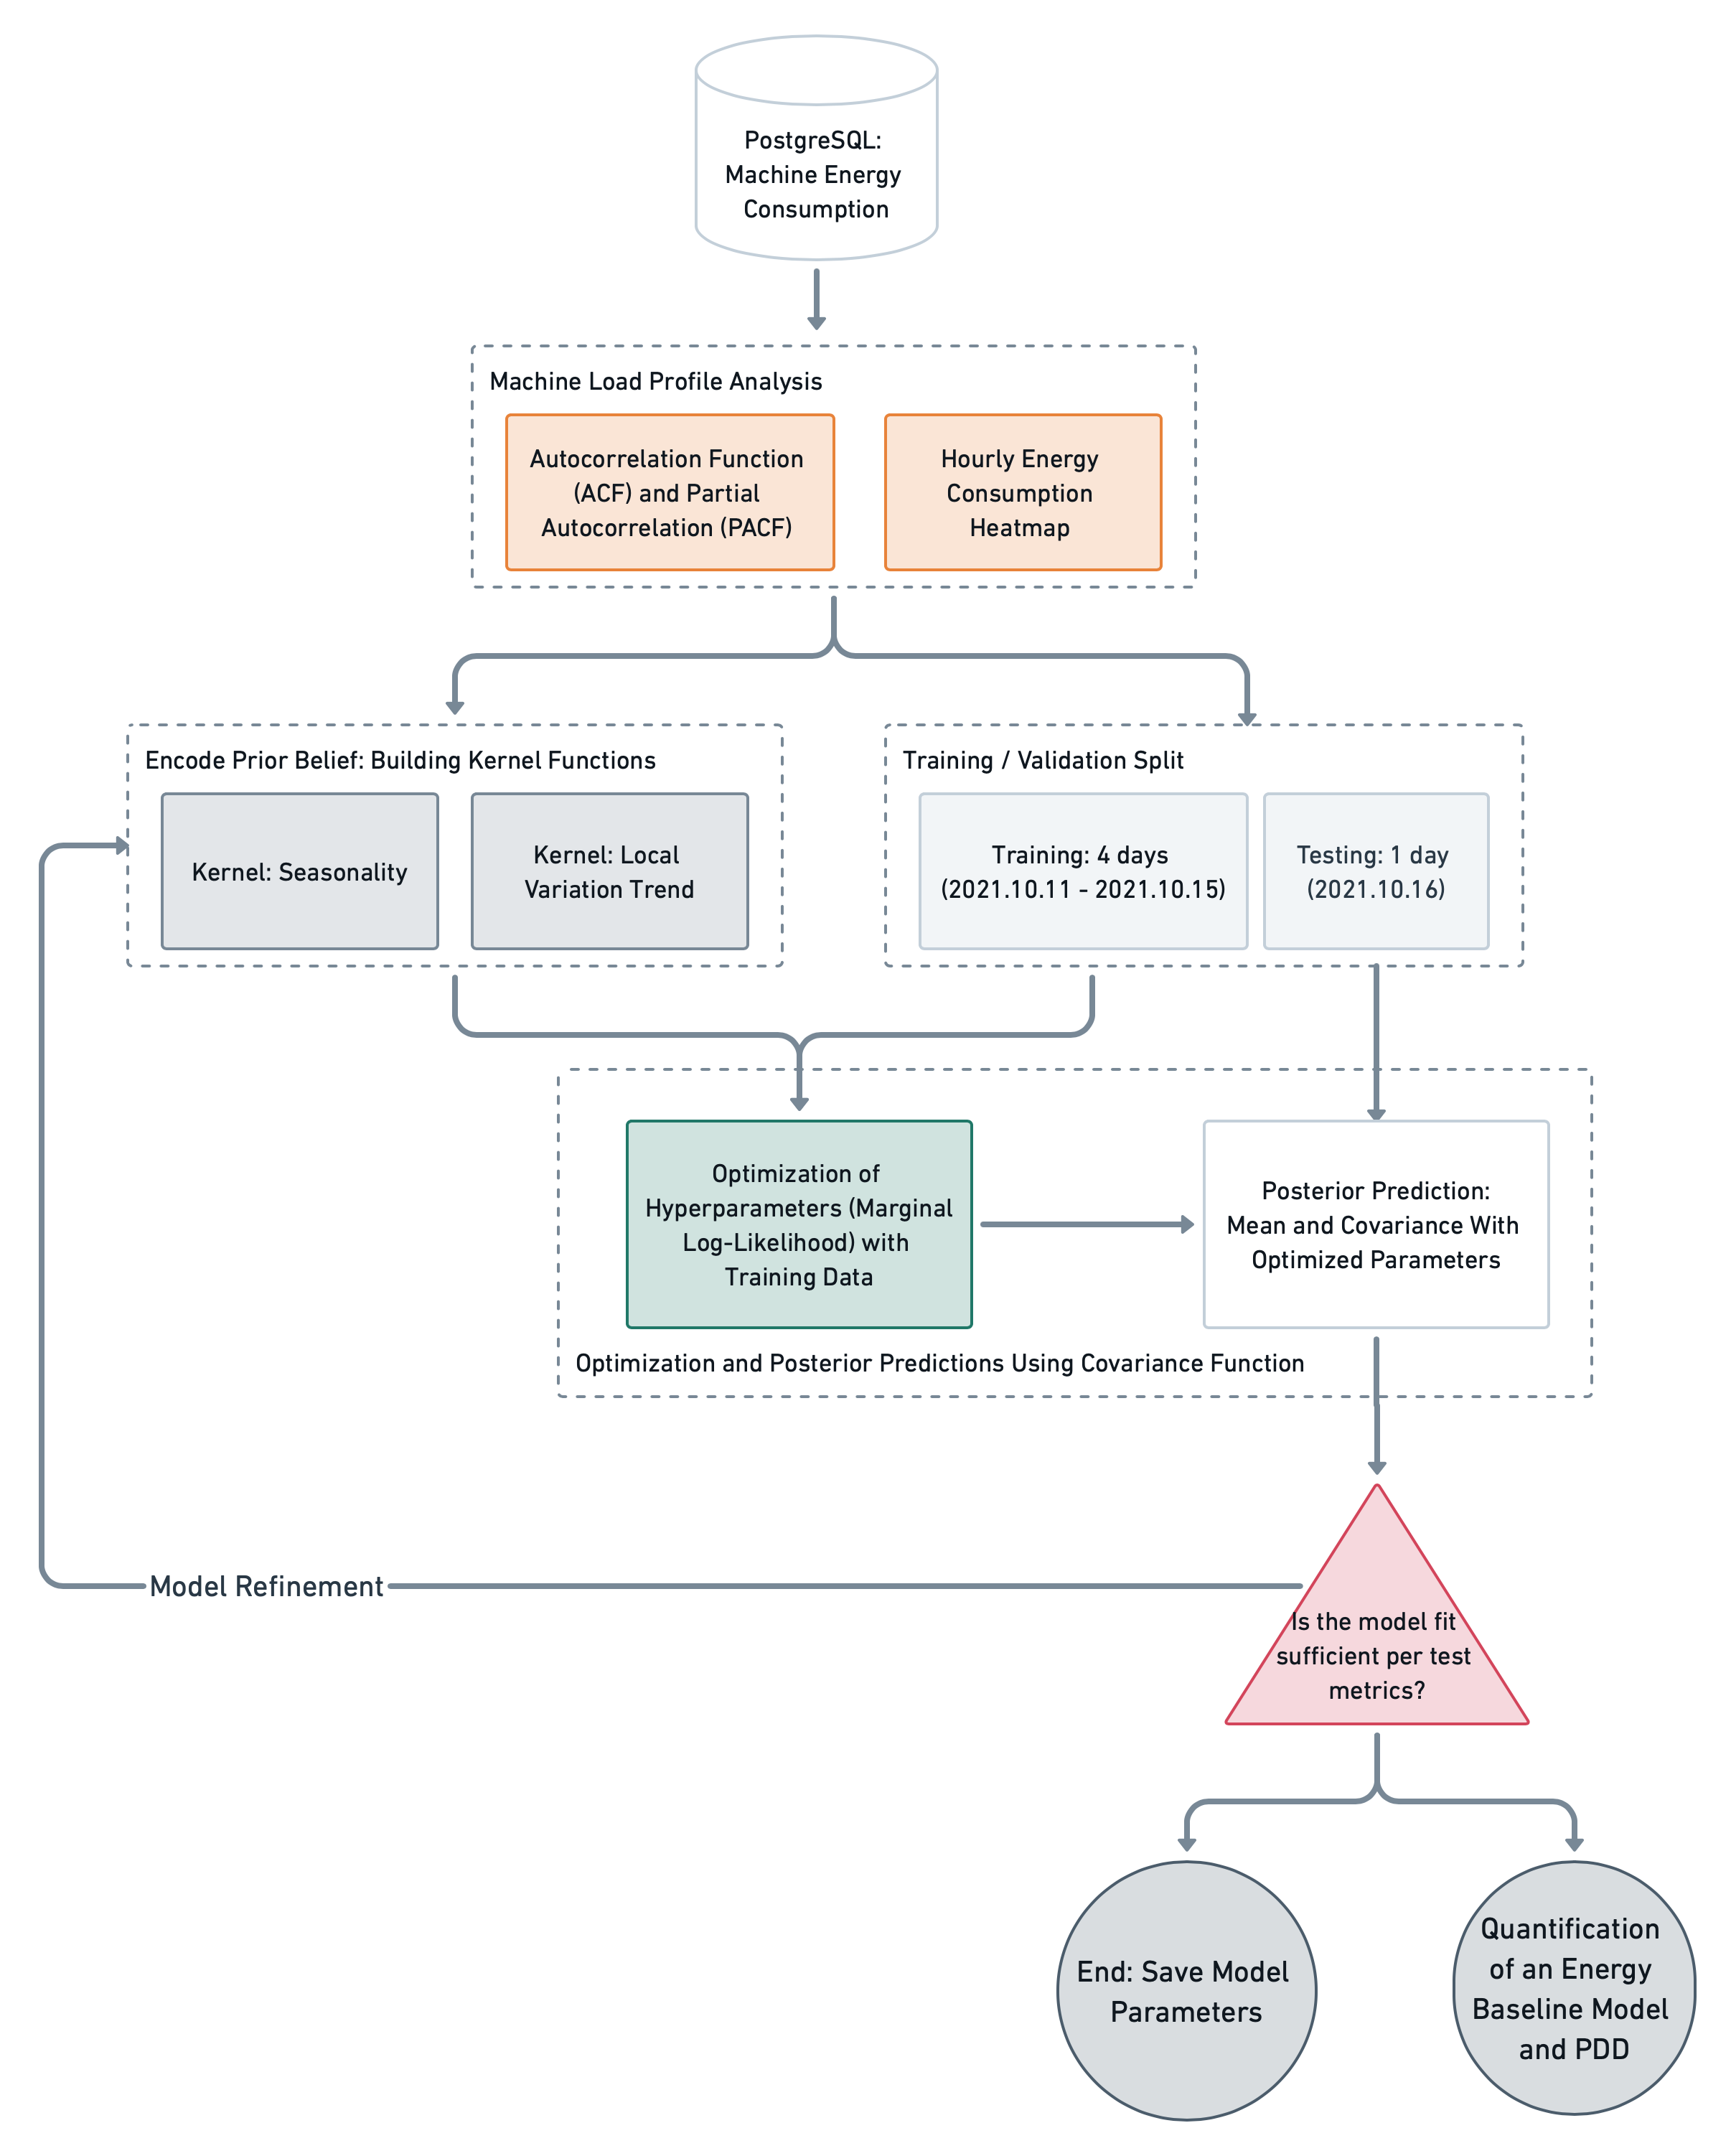
\includegraphics[scale=0.17]{images/experiment_flow.png}
\caption{Experimentation workflow for developing and refining energy baseline models.}
\end{figure}

\subsection{Model and Kernel Design, and Kernel Composition}

\subsection{Model Design Decomposition}

\subsection{Optimization and Cross Validation}

\subsection{Energy Baseline Model Experiment Performance Metrics}
\pagebreak

\section{Monitoring Energy Efficiency and Performance Deviation Detection using the Baseline Model}
\subsection{Evaluating Machine Energy Efficiency and Performance using Control Charts}

In this section, it is discussed on how to use the energy baseline model to identify a benchmark reporting period, monitor EE and perform PDD. Building off of \cite{oakland_statistical_2008}, the choice of the benchmark reporting period in which the model is trained on is crucial as it provides a reference to which predictions are compared to. In \cite{cas}, the authors trained their MLR on a period of one year and plotted the instantaneous and cumulative residuals. These two SPC charts allowed the authors to analyze periods of \textit{best} CAS performance indicated by the residuals fluctuating around a mean of zero. Ultimately, the baseline model was then retrained on a time period of $36$ days representing the \textit{best} performance. Here, an example of a workflow for choosing the benchmark reporting period for the paper disposal machine is given.

Using the kernel design according to the evaluation metrics in \hyperlink{table.3}{Table 3}, the model is trained on $10$ minute aggregated data from October $11^{th}$ until October $15^{th}$. In \hyperlink{figure.14}{Figure 14}, the top plot visualizes the instantaneous residuals of the in sample model fit. i.e., the difference of the predictions of the baseline model with the actual values of the benchmark reporting period. The bottom plot visualizes the cumulative residuals of the in sample fit. 

Where the SPC charts developed in this thesis differ from that in the literature and in industry is that the energy baseline model is a probabilistic model, and therefore, we have access to the uncertainty in our predictions. Where current SPC charts only take into account the point predictions and standard deviation of residuals to define UCL and LCL (as described in \hyperlink{subsection.2.3}{Section 2.3}), our proposed SPC charts utilizes the posterior distribution to define the control limits. Namely, by using the $95\%$ PI, a probabilistic approach can be used to determine the statistical significance of deviations in performance and change in EE over time. 

A red point in the top plot indicates that, at that time point $t$, the actual value was greater than $2 \sigma$ away from the mean prediction $\hat{\mu}_t$ and vice versa. Looking back at the time series plot in \hyperlink{figure.10}{Figure 10}, one can identify these outlier points. Then, in the CuSum plot, MA trend lines ($1$hr and $6$hr) are plotted to aid the identification of a benchmark reporting period. It can be seen that the slope of the residuals slightly increases until about the end of the day on October $12^{th}$, then is constant, and finally shows a slight decrease. However, in both charts, the mean of the residuals fluctuates around the zero bound, and thus the justification as using these four days for the benchmark reporting period is justified.

\begin{figure}[h]
\centering
\graphicspath{ {./images/} }
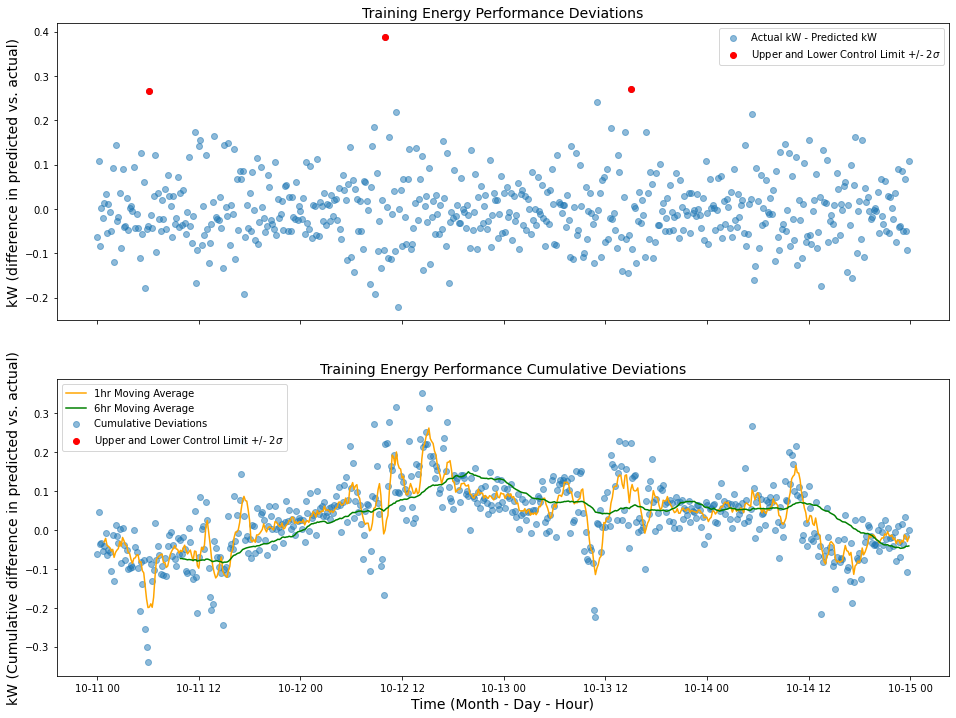
\includegraphics[scale=0.49]{images/entsorgung_baseline_SPC.png}
\caption{Entire time series for the paper disposal machine.}
\end{figure}

With a benchmark reporting period now chosen, predictions for every $10$ minutes for the next $24$ hours are computed. The same SPC charts are then visualized in \hyperlink{figure.15}{Figure 15} as a hypothetical example to what the operators / production leaders may receive in a real production environment. In the top chart, around 10:30a.m the paper disposal machine was consuming much less energy than what was deemed plausible by the GP model. Indicated by the red dots, these values lie in succession and are $2\sigma$ away from the expected value. Subsequently, there is a reversion back to what seems to be the nominal operating conditions. The CuSum plot, indicated by the change in slope starting at about 8:30a.m until 11:45a.m, identifies this deviation as a large deviation in machine energy consumption. With the SPC charts having identified a change in EE as a result of a significant decrease in energy consumption, the original time series is plotted again in \hyperlink{figure.16}{Figure 16}. Indeed, indicated by the red shading, there was a significant decrease in energy consumption. 

Furthermore, when a change in EE is identified, the time, machine, actual value, and degree of deviation (indicated by the z-score; how many standard deviations away a value is from the mean) is logged in a database where a historical registry of machine deviations can be built. Operations and maintenance teams can analyze this table to discuss each event, and the more data that is predicted and compared to the benchmark, the more valuable the registry becomes. For example, \hyperlink{figure.17}{Figure 17} refers to the deviations that occurred on 15.10.2021, the type of machine, and the degree of deviation. To communicate z-scores to a non-technical audience, a color coding scheme is used where red indicates the actual value landed $3\sigma$ away, yellow is $2\sigma$, and green is $1\sigma$. The arrows indicate in which direction the deviation occurred, i.e., an energy decrease or increase.


\begin{figure}[h]
\centering
\graphicspath{ {./images/} }
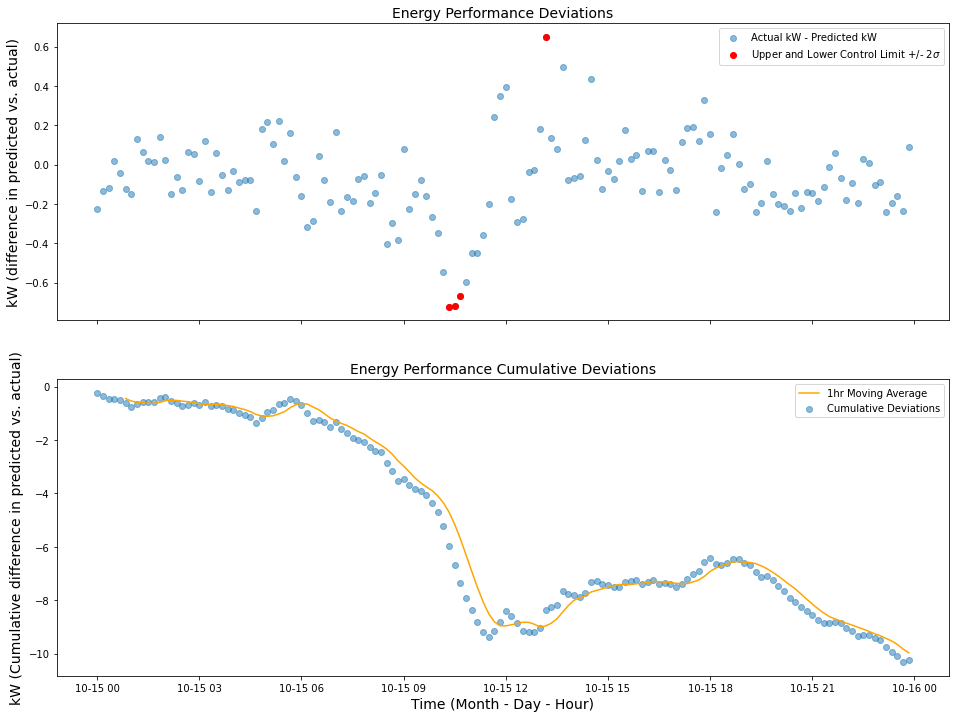
\includegraphics[scale=0.49]{images/entsorgung_test_SPC.png}
\caption{Using the test data, the paper disposal machine SPC charts are visualized. The top plot is the instantaneous residuals whereas the bottom is the CuSum of residuals.}
\end{figure}

\begin{figure}[h]
\centering
\graphicspath{ {./images/} }
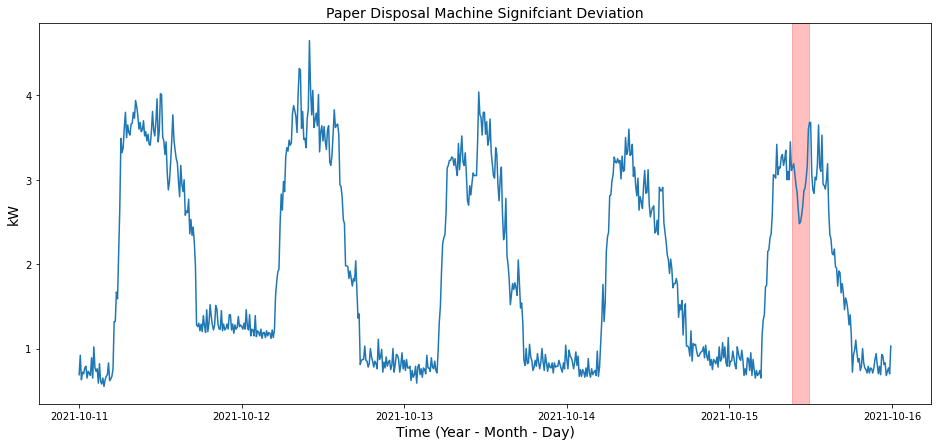
\includegraphics[scale=0.49]{images/entsorgung_deviation.png}
\caption{Original time series plotted for further analysis after the SPC charts and GP model identified a significant decrease in energy consumption indicated by the red shaded area.}
\end{figure}

\begin{figure}[h]
\centering
\graphicspath{ {./images/} }
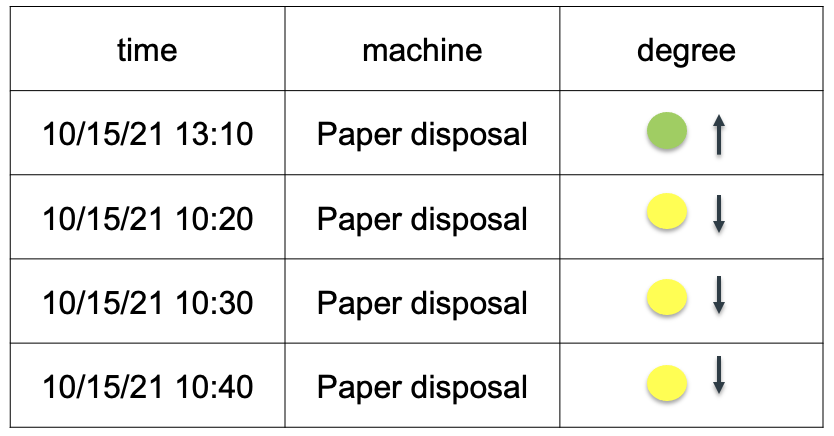
\includegraphics[scale=0.49]{images/entsorgung_registry.png}
\caption{Historical registry of paper disposal machine performance deviations. }
\end{figure}

\subsection{Mock Model Deployment}

Per the experimentation workflow in \hyperlink{figure.12}{Figure 12}, the final step is to save the model's parameters (state) to a \path{.pth} file. Within this file is the full "raw" state of the learned GPyTorch model parameters. Saving this to a file allows one to simply load the model's state back into an ExactGP module and perform inference without any further training needed. To prepare the GPyTorch model for a prototype deployment in CLEMAP's environment and infrastructure, the focus will be on developing a docker container for the \textit{inference} phase. As \hyperlink{figure.18}{Figure 18} shows, this consists only of the ExactGP module, model state, and kernel and utilities.

Docker + GitHub Actions

\subsection{Inspection of Learned Hyperparameters}

\subsection{Assumptions and Limitations of Models}

One of the assumptions of the models is the benchmark reporting period. Ideally, one should have a longer time period to analyze and to choose this period from. Indeed, most of the related work in \hyperlink{section.2}{Section 2} had access to several months of data. The work conducted in this thesis was meant to be an exploration / proof of feasibility, and therefore access to more data was limited. A longer time series allows for a wider range of production processes and periodicity's to be modeled than the current production week implemented in this thesis.

A limitation of the current baseline model implementation is that it does not take into account other covariates or production processes. Rather, it is only an extrapolation based on the past. For example, a meeting with CLEMAP's client production leader on 12.05.2022 had stated the company plans the next week's production on the Thursday before. Therefore, there is the possibility to include the production as a covariate for some of the models. However, this information came too late in this thesis to incorporate. Furthermore, after speaking with the production leader, it is clear the production processes are complex and can vary from order to order. The heterogeneous production environment makes it false positives more likely when changing production environments are not taken into account.
\pagebreak

\section{Conclusion}
\subsection{Summary of Main Results}

Using the metering data provided by CLEMAP, an energy consumption benchmark is established using a reporting period that represents the ``best operating conditions" for a piece of equipment and where the residuals fluctuate around a mean of zero. From there, using the posterior predictive distribution and SPC charts, the EE is monitored and analyzed to identify when a machine is deviating away from the expected behavior. Thus, not only is a probabilistic energy baseline model useful in benchmarking energy consumption, but it also provides value to the client in identifying a significant deviation in EE. As a proof of concept, an example was shown using the paper disposal machine. Using the methods proposed, the model and SPC charts identified a large decrease in energy consumption. When these charts were presented to the production leader and technician of CLEMAP's client, they had stated they were not too sure what could have caused such a significant decrease, but it could be related to the R707LV, XL106, or steel folding machine. Furthermore, when presented the time series plots, they were surprised that the machine was cycling over night, when in fact the machine should not be consuming energy.

For proof of feasibility, it was determined that a batch setting was the most cost effective way of developing the models. In a batch setting, the entire dataset $D$ is available before training starts. Therefore, this allowed CLEMAP to give us a ``data dump" which doesn't incur additional costs for the company in the form of increased technical support and compute. However, it is possible with CLEMAP's \ac{API} to develop the model in an online setting, i.e., the data arrives sequentially in an unbounded stream. Though, this type of modeling is more demanding in regard to compute power, API requests, and technical skillsets—all resulting in additional costs for CLEMAP. Subsequently, with several models having been developed for the proposed machines, a docker container is created in preparation for deployment on CLEMAP's infrastructure. This container represents the \textit{inference} phase, and allows CLEMAP to incorporate and or develop this container into their production environment as needed. 

\subsection{Comparisons and Differences to Current Research and Work in Industry}

In this thesis, methodologies currently in use in the industry were utilized and built on top of. Here, the comparisons and differences are outlined. Referring to \hyperlink{section.2}{Section 2}, additional data is often used to improve the quality of the model and to provide additional insights into the quantification of EE and PDD. Data is typically compiled through two forms: (1) additional sensors, and (2) non-sensor based. Per the meeting with CLEMAP's client on 12.05.2022, they have data on the week ahead production schedule and are interested in using this data—combined with the energy data—to produce productivity metrics. Likewise, this production data could be used as an input, in addition to the time input, in the GP to improve the quality of the energy baseline model. In doing so, the forecasted energy consumption would also be correlated with the expected produced goods. In \cite{HIPE} \cite{boiler} \cite{gas-turbine-faults}, data related to harmonic oscillations was also collected and used to quantify its relationship with energy consumption and deviations in EE. The probabilistic methods used in this thesis allows for the communication of uncertainty in the SPC charts and forecasted energy consumption using the posterior predictive distribution. Whereas in the literature, single point predictions are used which doesn't allow for a range of plausible values. 

\subsection{Applicability of Methods and Research to Other Contexts Within Industry 4.0}

In this thesis, benchmarking energy consumption and identifying deviations using an energy baseline model is a scalable framework that can be adapted to different machines in an industrial setting (as shown in \hyperlink{section.2}{Section 2} and with the analysis on the HIPE data). The specific method chosen for modeling in this thesis, namely Gaussian Processes, is also a powerful non-parametric way for modeling non-linear time series. The construction of kernels allows one to model a wide variety of processes. However, GPs have difficulty in extrapolating when the underlying physical process of a machine displays less evidence of a component(s) of a time series \hyperlink{subsection.3.2}{Section 3.2}. For example, the R707LV printer in Figure \ref{fig:fig19} of the appendix displays less evidence of cyclical patterns. Likewise, the underlying function has ``kinks" which is very difficult to model as most kernels generate smooth functions. Therefore, when the time series displays abrupt changes, i.e., kinks or discontinuities in the underlying function, GPs with the standard kernels presented in this thesis perform poorly in extrapolation. 

\subsection{Next Steps}

Next steps include leveraging the insights (incorporating production data) from the meeting on 12.05.2022 with CLEMAP's client to provide additional value to monitoring EE and performing PDD. Likewise, defining productivity metrics using the baseline model could be calculated. For example, using the expected amount of produced goods for the next production week, an energy consumption forecast could then be computed using the amount of produced goods as a covariate. From there, productivity metrics could be forecasted such as energy consumed per unit of produced good (output). Then, following the same framework in the thesis, the difference between the forecasted and actual value could be monitored to identify at which process or machine the productivity metric is deviating from the forecast. Another area of improvement is to define a longer reporting period than four production days. The current four days may include some latent variable that is not accounted for, and therefore it is suggested to use a longer time series to train the GP model to analyze potentially different consumption profiles as in \cite{cas}. 



\pagebreak

\section{References}
\printbibliography[heading=none]
\pagebreak

\appendix
\section{Appendix}
This appendix contains figures that do not flow and or belong in the main body of the thesis. Figure \ref{fig:fig18} is the result of a Gaussian Process model fit and predictions for the main terminal. Figure \ref{fig:fig19} is the production week time series for the R707LV printer. 


\begin{figure}[h]
\centering
\graphicspath{ {./images/} }
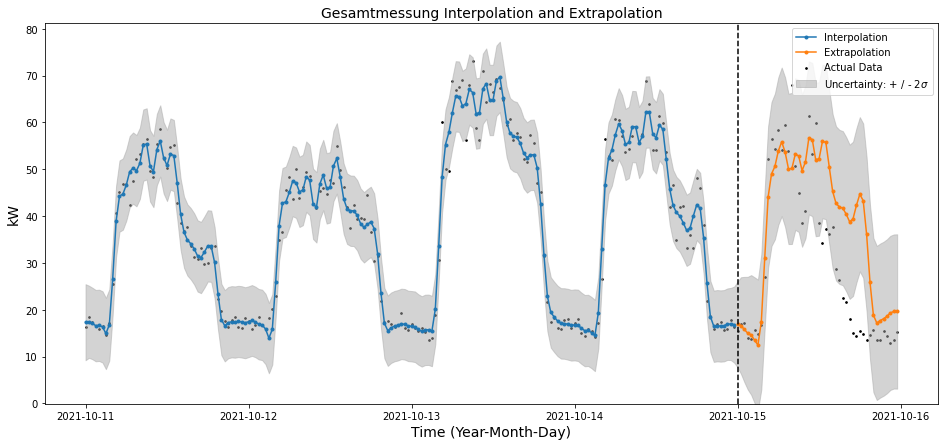
\includegraphics[scale=0.49]{images/gesamtmessung_model.png}
\caption{Interpolation and extrapolation for the main terminal GP model at a $30$ minute time aggregation. The demand for energy during the afternoon on Friday tapered off much quicker than what the baseline model had predicted and thus is the reason for the poor evaluation metrics.}
\label{fig:fig18}
\end{figure}


\begin{figure}[H]
\centering
\graphicspath{ {./images/} }
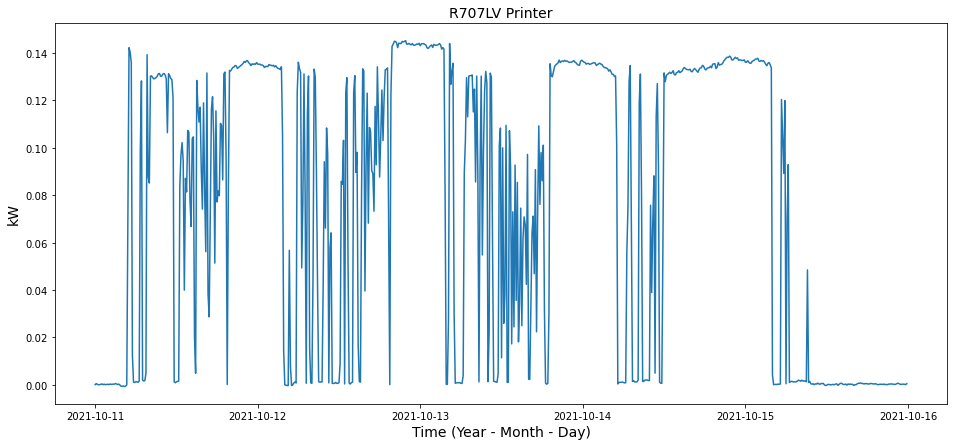
\includegraphics[scale=0.49]{images/r707lv_printer.png}
\caption{$10$ minute frequency of the R707LV printer displays some periodicity but is not identifiable by the ACF correlogram and $Per$ kernel.}
\label{fig:fig19}
\end{figure}


\pagebreak

``I hereby confirm that I \underline{\hspace{10cm}}:
\begin{itemize}
    \item have written this Thesis independently and without the help of any third party.
    \item have provided all the sources and cited all the literature I used.
    \item will protect the confidentiality of the client and respect the copyright regulations of Lucerne University of Applied Sciences and Arts."
\end{itemize}

\end{document}